%\documentclass[a4paper]{article}
\documentclass[10pt,a4paper]{article}
\usepackage[utf8]{inputenc} % para poder usar tildes en archivos UTF-8
\usepackage[spanish,es-tabla]{babel}
\usepackage{verbatim}
\usepackage{clrscode3e}
\usepackage{amssymb}
\usepackage{graphicx}
\usepackage{float}
\usepackage{pdfpages}
\usepackage{subcaption} %  for subfigures environments 


% \usepackage{bibtex}

%\usepackage{a4wide} % márgenes un poco más anchos que lo usual

\usepackage{caratula} % Se puede descargar en ~> https://github.com/bcardiff/dc-tex
\usepackage[breaklinks=true]{hyperref}


\begin{document} % Todo lo que escribamos a partir de aca va a aparecer en el documento.

%fran
%\sloppy

% Completar los datos de la caratula
\titulo{Trabajo Práctico 2 - Reconocimiento de Imagenes} 
\fecha{\today}
\materia{Métodos Numéricos}
\grupo{Grupo "Greco - Herrera - Kubrak"}

% Completar los integrantes del grupo:)
%\integrante{Facundo, Araujo}{321/15}{facalj\_velez@hotmail.com}
\integrante{Cristian, Kubrak}{456/15}{Kubrakcristian@gmail.com}
\integrante{Marcela Alejandra, Herrera}{1162/84}{marcelaalejandraherrera@yahoo.com.ar}
\integrante{Luis Fernando, Greco}{150/15}{luifergreco@gmail.com}


\maketitle
\par \textbf{Abstract:} El objetivo del Trabajo es realizar reconocimiento de imágenes de rostros mediante aprendizaje supervisado. 
\par Se utiliza K-fold cross validation para generar las muestras de prueba y de validación a partir de la base de datos disponible. Durante la fase de reconocimiento se utiliza KNN para determinar a qué individuo pertenece la imagen. Como técnica auxiliar para preprocesar las imágenes se aplica PCA como forma de optimizar el uso del espacio de almacenamiento. Para la obtención de las componentes principales en PCA se utiliza el algoritmo de Deflación.
\par Para la evaluación de los resultados se utilizan las métricas de accuracy y recall.

\par  \textbf{Palabras clave:} Reconocimiento de rostros - Aprendizaje supervisado - PCA - KNN - KFold - Método de la potencia - Algoritmo de deflación - Accuracy - Recall.


% Aca comienzan a escribir su informe
\tableofcontents

\newpage

\section{Introducción}
\subsubsection*{Introducción}
\par El problema que se nos plantea es el de realizar un reconocimiento facial mediante aprendizaje supervisado. Partimos de una base de datos, a la cual llamamos \textit{base de entrenamiento},
que consiste en fotografías de un conjunto de $N$ personas de las cuales contamos con $M$ fotos diferentes de las caras de cada una. Al recibir una nueva imagen, buscamos identificar a qu\'e persona le corresponde. 
\par Para reconocer la nueva cara experimentamos con dos m\'etodos: el primero usando los $k$ vecinos m\'as cercanos (\textit{kNN}) y el segundo utilizando el an\'alisis de componentes principales (\textit{PCA}) como forma de preprocesar la \textit{base de entrenamiento} para reducir el tama\~{n}o de la imagen y luego utilizar \textit{kNN} sobre la base preprocesada. 
\par Por \'ultimo, para evaluar los m\'etodos y la correcta elecci\'on de par\'ametros utilizamos una t\'ecnica de \textit{cross validation} llamada \textit{K-fold}.

\subsubsection*{K vecinos m\'as cercanos}
\par A partir de la \textit{base de entrenamiento} buscamos identificar a qu\'e sujeto pertenece una nueva cara sin identificar. Asumimos que todas las imágenes son del mismo tamaño y las representamos por medio de un vector de dimensi\'on $m$, donde $m = altura*ancho$ (medidos en pixeles). Para cada imagen además conocemos su ID (i.e.: identificador que nos permite saber a qué persona corresponde la imagen).
\par Mediante el c\'alculo de la norma de la diferencia entre los vectores de imagen, obtenemos los $k$ elementos m\'as cercanos, donde \textit{k} es un parámetro de experimentación.\\
Esta forma de encarar el problema resulta poco pr\'actica cuando la dimensi\'on de la im\'agen es grande, es por esto que en ciertos casos preprocesamos la base de datos con el m\'etodo \textit{PCA}.

\subsubsection*{An\'alisis de componentes principales}
Lo que se busca aplicando este método es disminuir la dimensión de la muestra, trabajando con menos variables que contengan información más representativa.
\par La cantidad de componentes con los que se va a trabajar es una parámetro de la experimentación, al cual denominamos $\alpha$.
\par Partiendo de las imágenes vectorizadas según se explicó en la sección \textbf{ K vecinos m\'as cercanos}, se arma una matriz que llamamos $I$, la cual contiene una imagen por fila, la misma tiene dimensión $n*m$ ($n$ cantidad de imágenes, $m$ cantidad de pixeles de cada imagen). En general esta matriz será rectangular con muchas más columnas que filas.
\par Para este algoritmo de preprocesamiento, se calcula el promedio de todas la im\'agenes: $\mu = (\sum_{i=1}^{n}I_{i})/n$ .
\par Luego se define la matriz $X \in {\rm I\!R}^{nxm}$, que en i-\'esima fila tiene al vector $(x_i -  \mu)/\sqrt{n -1}$. Si la base de entrenamiento cuenta con $n$ imágenes diferentes, y cada imagen tiene $m$ pixeles, la matriz $X$ tiene dimensión $n*m$.
\par Para esta matriz $X$, se debe calcular la matriz de covarianza definida como $M = X^tX$, de dimensión $m*m$.
\par Sea $v_j$ el autovector de $M$ asociado al j-\'esimo autovalor (teniendo los autovalores ordenados seg\'un su valor absoluto), se define para cada
$i = 1,..,n$ la \textit{transformaci\'on caracter\'istica} de $x_i$ como el vector $tc(x_i) = (v_1x_i,v_2x_2,..,v_\alpha x_i)^t \in {\rm I\!R}^\alpha$,
donde $\alpha$ es un par\'ametro de experimentaci\'on.\\
\par Por motivos de optimización, en este trabajo en vez de calcular la matriz de $M$, calculamos una matriz $\tilde{M} = XX^t$ de dimensión $n*n$ para luego mediante un cambio de variable
recuperar los autovectores de $M$.
\par Esto se puede realizar gracias a que ambas matrices poseen los mismos autovalores y los autovectores de una se pueden averiguar a partir de los de la otra.
\par Si $V$ es una base de autovectores de $\tilde{M} = XX^t$, $\sigma^2_{i}$ el autovalor asociado al autovector $v_i$, $U$ una base de autovectores de $M = X^tX$ con $u_i$ el autovector asociado al i\-ésimo autovalor (ordenados de mayor módulo a menor módulo), se pueden obtener los autovectores de $XX^t$ aplicando la siguiente fórmula: $u_i = \frac{A*v_i}{\sigma_i}$.

\subsubsection*{Cross validation} 
\par Para evaluar qu\'e tan bien funciona nuestro algoritmo es necesario realizar una validaci\'on de los resultados. Para esta tarea ultilizamos el m\'etodo de \textit{Cross validation} llamado \textit{k-fold}. \par Se subdivide la \textit{base de entrenamiento} en $k$ subconjuntos con igual cantidad
de elementos. Uno de estos subconjuntos lo utilizamos como datos de prueba mientras que los $k-1$ restantes constituyen la \textit{base de entrenamiento}. A partir de esto
podemos analizar los resultados ya que contamos con la informaci\'on respecto a qu\'e sujeto pertenece cada imagen de nuestra base de pruebas.
\par Por \'ultimo resta repetir
el procedimiento para que cada uno de los subconjuntos sea considerado como base de pruebas.

\subsubsection*{Criterios de evaluaci\'on}
Resulta de vital importancia tener en claro cu\'ales son los criterios a tener en cuenta para ver si nuestra clasificaci\'on es \textit{buena} o no.
Para poder evaluarla, debemos mirar los \textit{true positives} y \textit{true negatives} (los casos en los cuales el encasillado funcion\'o correctamente)
como tambi\'en los \textit{false positives} y \textit{false negatives} (casos en los cuales la clasificaci\'on no se comport\'o como se esperaba).\\
Siendo el caso a analizar no binario (existen m\'as de dos categor\'ias), para cada $i = 1,..,n$  definimos $tp_i$ como
las muestras que realmente pertenecen a la clase $i$ y fueron exitosamente identificadas como tales
y $fn_i$ son aquellas muestras que son identificadas como pertenecientes a la clase i cuando realmente no lo son (an\'alogamente definimos $tn_i$ y $fp_i$).
\par A partir de esto definimos cuatro m\'etricas, a saber:
$precision_i= \frac{tp_i}{tp_i + fp_i}$ la cual indica qu\'e porcentaje de los datos recuperados cu\'ales son relevantes. 
El $recall_i= \frac{tp_i}{tp_i + fn_i}$, que indica qu\'e porcentaje de los datos relevantes fueron recuperados.
El $accuracy_i = \frac{tp_i+tn_i}{tp_i + tn_i + fp_i + fn_i}$ indica la cantidad de aciertos sobre el total de la base de datos.
Por \'ultimo la media arm\'onica $F_{1_i} = 2\frac{precision_i * recall_i}{precision_i + recall_i}$ permite establecer un compromiso entre en 
$recall_i$ y el $accuracy_i$.

\subsubsection*{Método de la Potencia y algoritmo de Deflación}
\par El método de la potencia permite averiguar el autovalor de mayor módulo de una matriz y su autovector asociado.
\par Si la matriz en estudio posee una base ortonormal de autovectores y autovalores distintos, utilizando repetidamente el método de la potencia se pueden averiguar todos los autovalores, comenzando desde el de mayor módulo en orden decreciente y los autovectores asociados. Este mecanismo es el algoritmo de Deflación.
\par En el caso de la matriz $XX^{t}$ que utilizamos en este trabajo, se puede garantizar que se encuentra dentro de las hipótesis requeridas por el método de Deflación porque se trata de una matriz simétrica.

\newpage

% \section{Demostraciones}
% \newpage

\section{Desarrollo}
%\subsubsection*{Desarrollo}

%\textbf{Generalidades}
\subsection*{Generalidades}

Para experimentar analizamos la influencia en los resultados de las diferentes variables de experimentación que manejamos utilizando tanto el método KNN como el KNN + PCA. 
Las mismas son la cantidad de vecinos considerados por KNN (k), y la cantidad de componentes principales de la imagen transformada ($\alpha$).
Lo hicimos sobre dos bases de datos: una con im\'agenes de tamaño reducido, y otra con imágenes sin reducir.
Para manejar las imágenes implementamos la clase Imagen, en la cual almacenamos la imagen y demás parámetros necesarios de cada una de ellas.
Para la lectura de los archivos de imágenes utilizamos las librerías provistas por la cátedra.
Cada imagen leída se vectoriza, y con el conjunto de imágenes vectorizadas se arma una estructura matricial, que resultó práctica para la implementación de los algoritmos requeridos.

%\textbf{KNN}
\subsection*{KNN}

El KNN es de algúna forma el centro del desarrollo, ya que es donde se toma la decisión de cuál es el sujeto de la base de entrenamiento que se corresponde con la imagen que elegimos para testear.

Esto lo hicimos calculando la distancia euclídea entre el elemento a testear y todos los elementos de la base de entrenamiento, guardando la distancia resultante y el sujeto al que pertenecía cada imagen de la base. Luego ordenamos los datos de acuerdo a las distancias obtenidas. Con los datos ya ordenados tomamos los id correspondientes a las k menores distancias y finalmente calculamos la moda, es decir, el ID que  aparecía más veces. En otras palabras quién es el individuo que "matchea" mejor con la imagen que testeamos según nuestros métodos. 

\par Una de las dificultades con que nos encontramos fue el decidir los tipos de datos a utilizar. Las imágenes vienen codificadas con números enteros entre 0 y 255 y para trabajar con KNN (sin PCA) utilizamos enteros que ocupan menos espacio de memoria. Sin embargo por la naturaleza de los cálculos necesarios para PCA tuvimos que utilizar doubles. Esto nos llevó a tener que duplicar parte del código para adaptarse al nuevo tipo de dato.


%\textbf{PCA}
\subsection*{PCA}
La implementación del método PCA consta de varios pasos:
En un primer paso se arma la matriz X (de tipo matriz de doubles) que contiene los bytes de datos de las imágenes vectorizadas. Esta matriz se debería usar para calcular la matriz de covarianza de la muestra, que luego debería ser diagonalizada para obtener los autovectores que permiten hacer una cambio de base de la muestra dejando las variables (valores de las columnas) lo más independientes posible.
La matriz de covarianza se calcula haciendo el producto matricial $X^{t} * X$. Considerando que la cantidad de columnas de la matriz $X$ es igual a la cantidad de pixeles de una imagen, el resultado del producto es una matriz que fácilmente puede volverse gigantesca como para poder operar con ella, de manera que resulta muy costoso en términos de uso de la memoria del equipo. Con el objeto de atenuar este problema, en lugar de calcular los autovectores de la matriz $X^{t} * X$, lo hacemos con $X * X^{t}$.
\par Estas matrices comparten los mismos autovalores y sus autovectores puede ser calculados unos en función de los otros, tal como se detalla en la Introducción teórica. Si bien la implementación se complicó porque tuvimos que programar la conversión de los autovectores, la ventaja que obtuvimos es que operamos con matrices de menor dimensión, puesto que la cantidad de imágenes (filas de X) es en nuestro caso notablemente menor que la cantidad de pixeles de cada imagen (columnas de X).
La matriz $X * X^{t}$ es una matriz simétrica, en un principio nos planteamos la posibilidad de usar alguna estrategia de almacenamiento que aprovechara esta condición para ahorrar memoria, pero en este caso decidimos no hacerlo y tratarla como una matriz común para simplificar la implementación, sin embargo en caso de una implementación donde sea crítico el uso del espacio debería considerarse seriamente esta opción.

\subsection*{Método de la potencia}
El método de la Potencia necesita para la iteración de un vector $x$ que inicialmente contiene un valor arbitrario, el cual decidimos generar de forma aleatoria. Durante el testeo de las funciones observamos que corridas sucesivas efectuadas con las mismas imágenes de entrada producían diferentes resultados en los autovectores generados. Las diferencias se observan en los decimales menos significativos. La hipótesis es que estas diferencias se producen por utilizar el vector inicial generado de manera aleatoria. Si bien esta forma de generarlo sirvió muy bien a la hora de calcular los autovalores y autovectores de la matriz de covarianza, no resulta bueno a la hora de reproducir los experimentos, algo de lo que nos dimos cuenta luego de la experimentación.
\par En el método de Deflación pudimos observar que al buscar autovalores y autovectores, las componentes principales tienen una convergencia más veloz, arribándose a un resultado preciso en pocas iteraciones del método de Potencia. A medida que se calculan mayor cantidad de componentes, la convergencia del método de Potencia se hace notoriamente más lenta y por momentos parecía que no había convergencia cuando en realidad sí la había. Esto nos llevó a utilizar dos criterios de parada para el cálculo de cada autovalor: en una primera instancia usamos una cantidad de iteraciones tope de 10.000, pidiendo una variación entre los resultados de dos iteraciones sucesivas menor a $10^{-5}$; si al cabo de 10.000 iteraciones no llegamos a una convergencia, continuamos iterando hasta un tope de 100.000 iteraciones más y aceptando una tolerancia menos precisa de $10^{-3}$.


\subsection*{Kfold (Cross-validation)}
Decidimos utilizar 5-fold.
La determinación del valor de $k$ la realizamos teniendo en cuenta los siguientes factores:
\begin{itemize}
\item Al realizar la partición de la base de datos en datos de entrenamiento y datos de test queríamos que cada clase estuviera representada en una proporción similar, o sea que la selección fuera balanceada. Si bien al principio habíamos pensado hacer la partición de forma aleatoria, esto hubiera podido llevar a situaciones como por ejemplo tener en la base de entrenamiento todos los elementos de una clase y muy pocos de otra con lo cual el entrenamiento sería sesgado favoreciendo a la clase con más representantes. Por otro lado a la hora de testear podría no haber elementos de esa clase que no hubieran sido usados para entrenar con lo cual se invalidarían los resultados. Contrariamente los parámetros elegidos podrían no ser adecuados para la clase con menos representantes, con lo cual el reconocimientos de elementos pertenecientes a esa clase sería deficiente.

\item Teniendo en cuenta el punto anterior los posibles $k$ elegibles se reducen a los divisores de la cantidad de imágenes de cada clase. Siendo en el nuestro caso de 10 imágenes por clase los posibles valores son: 1, 2, 5 y 10. El 1 no tiene sentido en la práctica ya que equivale a no tener datos de entrenamiento. El 10 supone que queda solo un representante de cada clase para testear, entonces si la imagen que usamos para testear posee algúna anormalidad respecto de las otras de su clase afectaría negativamente nuestros resultados, es decir, nuestro resultado sería muy sensible a outsiders y poco robusto. En el caso de 2, estaríamos usando la mitad de los datos para entrenar y la mitad de los datos para testear y tratándose de una base de datos relativamente chica (con pocos representantes de cada clase) consideramos que tendríamos poca variedad de datos de entrenamiento. En el caso de $k$=5, estaríamos considerando dos imágenes de cada clase para testear y ocho para entrenar. De todas las posibilidades, nos pareció la más adecuada porque nos da una cantidad relativamente grande de datos de entrenamiento y más de una imagen para testear. 
\end{itemize}

\subsection*{Métricas}

\par Las métricas que elegimos para evaluar los resultados fueron \textit{accuracy} y \textit{recall}, con el \textit{accuracy} tenemos una medida de clasificaciones correctas en general (o sea las veces que se acierta en clasificar en la clase correcta y en no clasificar en una clase que no corresponde), mientras que el \textit{recall} nos permite maximizar la cantidad de identificaciones acertadas de cada clase en relación al total de elementos de la clase presentes en la muestra.
Para calcularlas, por cada fold, para cada imagen a reconocer se guarda el ID de la clase a la que pertenece y la clasificación que hace el sistema.
\par Una vez obtenida esta información para todas las imágenes a reconocer de la totalidad de los folds, se procede a calcular los verdaderos positivos, verdaderos negativos, falsos positivos y falsos negativos. Y con estos se calculan las métricas mencionadas (como se detalló en la introducción teórica).

\subsection*{Experimentación}

%\textbf{Experimentación}
\par Uno de los parámetros determinantes en la experimentación es la cantidad de vecinos cercanos, otro punto relevante es el valor de $\alpha$ que vamos a utilizar. Es por eso que vamos a plantear una serie de tests con estos parámetros para determinar los valores que nos ofrezcan un mejor \textit{trade off} entre las diferentes métricas que utilizaremos para evaluar nuestra implementación.\newline
Estas son Accuracy, Recall y el tiempo de ejecución.

A su vez, vamos a testear lo mencionado anteriormente tanto con la implementación de KNN como con KNN+PCA para evaluar también el funcionamiento de PCA. 

Nota: En los tests dónde evaluamos $\alpha$ tomamos K = 1 y de la misma forma, en los que evaluamos K tomamos $\alpha$ = 10. 

\par Nuestras expectativas previas a la experimentación son las siguientes:\\
Por un lado consideramos que el tamaño de las im\'agenes influirá acrecentando el tiempo requerido para su procesamiento pero debido a la mayor informaci\'on disponible, con las imágenes más grandes 
funcionarán mejor los algoritmos.\\
Con respecto a la variaci\'on del $k$ en $KNN$ suponemos que los mejores resultados de reconocimiento los tendremos con un $k$ no demasiado grande.\\
Frente a los diferentes algoritmos (KNN o PCA + KNN) creemos que la segunda opci\'on realizar\'a un mejor trabajo pero a su vez requiere de un mayor tiempo para el preprocesamiento de las imágenes, aunque el tiempo de reconocimiento suponemos que debería ser similar o menor que en knn solo.
Por \'ultimo, respecto al par\'ametro $\alpha$ (cantidad de iteraciones del m\'etodo de las potencias) resulta obvio estimar que a mayor $\alpha$, mayor ser\'a el tiempo de ejecución aunque como contrapartida esperamos que un mayor $\alpha$ mejore significativamente la tasa de reconocimiento.


\newpage

\section{Experimentación}
\subsubsection*{Experimentación}
Para experimentar analizamos la influencia en los resultados de las diferentes variables de experimentación que manejamos utilizando tanto el método KNN como el KNN + PCA. 
Las mismas son la cantidad de vecinos considerados por KNN (k), y la cantidad de componentes principales de la imagen transformada ($\alpha$).
Lo hicimos sobre dos bases de datos: una con im\'agenes de tamaño reducido, y otra con imágenes sin reducir (a las cuales llamaremos \textit{big tempo})
Nuestras expectativas previas a la experimentación fueron las siguientes\\
Por un lado consideramos que el tamaño de las im\'agenes influir\'a en el tiempo requerido para su procesamiento pero debido a la mayor informaci\'on disponible,
funciar\'an mejores los algoritmos.\\
Con respecto a la variaci\'on del $k$ en $KNN$ suponemos que con un $k$ ni muy grande ni muy chico, obtendremos buenos resulatados de reconocimiento.\\
Frente a los diferentes algoritmos (KNN o PCA + KNN) creemos que la segunda opci\'on realizar\'a un mejor trabajo pero en un mayor tiempo, por lo que habr\'a que evaluar si se justifica su utilizanci\'on.\\
Por \'ultimo, respecto al par\'ametro $\alpha$ (cantidad de iteraciones del m\'etodo de las potencias) resulta obvio estimar que a mayor $\alpha$, mayor ser\'a el tiempo de ejecuc\'on aunque esperamos que esto
mejore significativamente la tasa de reconocimiento.

\newpage

\section{Resultados}


\subsubsection*{Resultados obtenidos}
%Nota: Al ser los resultados de los experimentos sobre ambos tests muy similares, decidimos analizarlos en conjunto.

Uno de los parámetros determinantes en la experimentación es la cantidad de vecinos cercanos, otro punto relevante es el valor de $\alpha$ que vamos a utilizar. Es por eso que vamos a plantear una serie de tests con estos parámetros para determinar los valores que nos ofrezcan un mejor \textit{trade off} entre las diferentes métricas que utilizaremos para evaluar nuestra implementación.\newline
Estas son Accuracy, Recall y el tiempo de ejecución.

A su vez, vamos a testear lo mencionado anteriormente tanto con la implementación de KNN como con KNN+PCA para evaluar también el funcionamiento de PCA. 

Nota: En los tests dónde evaluamos $\alpha$ tomamos K = 1 y de la misma forma, en los que evaluamos K tomamos $\alpha$ = 10. 
\subsubsection*{Tests KNN}

\begin{figure}[H]
\begin{subfigure}[h]{0.62\linewidth}
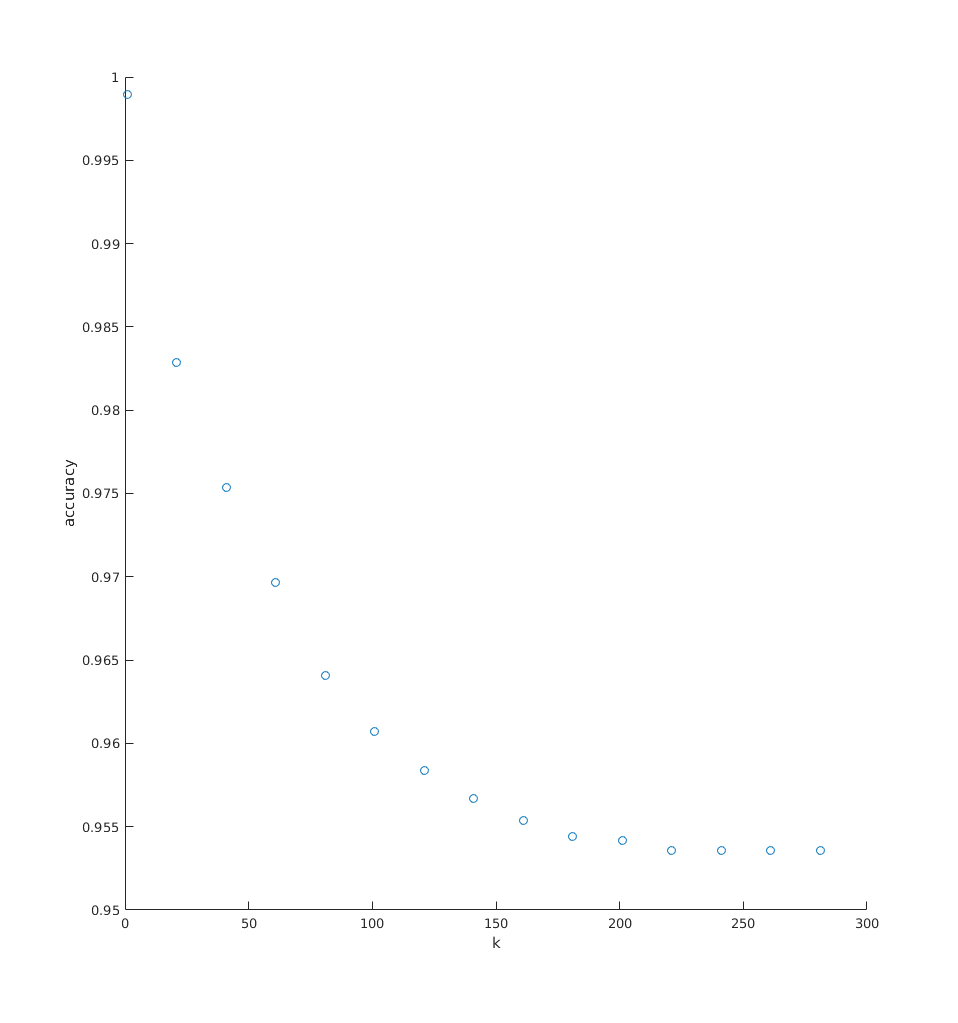
\includegraphics[width=\linewidth]{img/k_knn_accu.png}
\caption{Utilizando imágenes reducidas}
\end{subfigure}
\hfill
\begin{subfigure}[h]{0.62\linewidth}
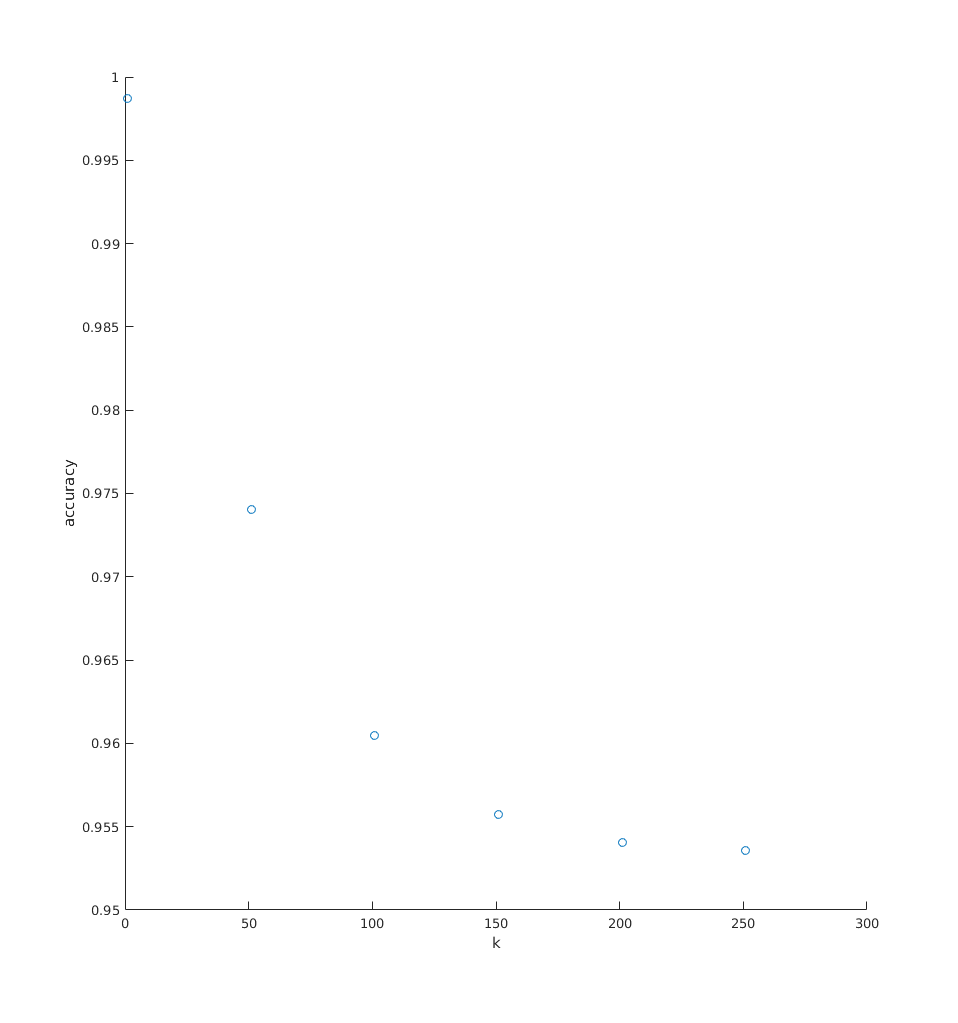
\includegraphics[width=\linewidth]{img/big_k_knn_accu.png}
\caption{Utilizando imágenes grandes}
\end{subfigure}%
\caption{K vs Accuracy con KNN sin PCA}
\end{figure}

En ambos casos obtenemos resultados similares, un Accuracy más grande a menor K, siendo K = 1 el valor óptimo, al menos en este caso.
%Dados los resultados, en este caso consideramos que utilizando un valor de K cercano a 10 obtenemos la mejor relación (dentro de nuestro set de tests).\newline
%Por un lado evitamos el problema que ocurre cuando K es demasiado grande y por otro, tomamos una cantidad de imágenes cercanas suficiente como para minimizar el impacto de algún outsider. Aun que cabe destacar que en este caso particular K = 1 tuvo un mejor comportamiento de lo que esperabamos, consideramos que sería arriesgado tomarlo como valor confiable con otros sets de imágenes.

%%%%%%%%%%%%%%%%%%%%%%%%%%%%%%%%%%%%%%%%%%%%%%%%%%%%%%%%%%%%%%%%%%%%%

\begin{figure}[H]
	\centering
	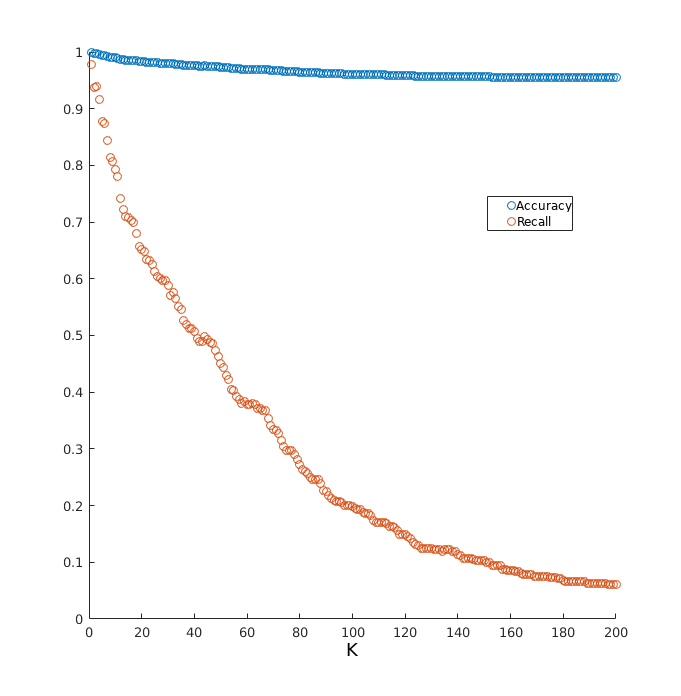
\includegraphics[width=0.8\textwidth]{img/Acc_recall_k_knn.png}
	\caption{Accuracy y Recall vs K (sin PCA)}
	\label{fig: Accuracy y Recall vs K (sin PCA)}
\end{figure}

En este gráfico encontramos algo similar al anterior, si bien se nota un descenso en Accuracy a medida que aumenta K, con el cambio de escala se puede apreciar que el mismo es muy leve.
Por el contrario, sí encontramos que Recall disminuye considerablemente a medida que K crece. En este caso es esta métrica la que nos da más elementos para concluir que K = 1 es la mejor opción.


%%%%%%%%%%%%%%%%%%%%%%%%%%%%%%%%%%%%%%%%%%%%%%%%%%%%%%%%%%%%%%%%%%%%%


%%%%%%%%%%%%%%%%%%%%%%%%%%%%%%%%%%%%%%%%%%%%%%%%%%%%%%%%%%%%%%%%%%%%%
%\begin{figure}[H]
%	\centering	
%	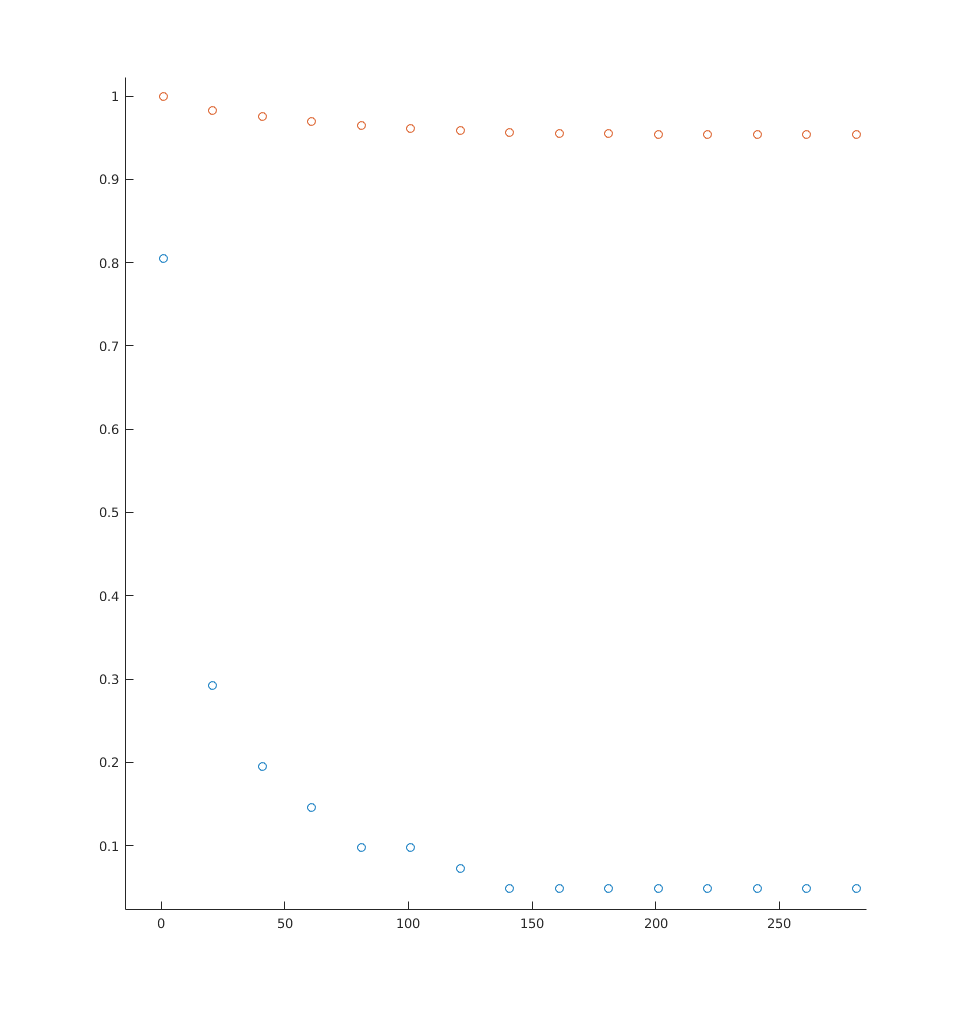
\includegraphics[width=0.8\textwidth]{img/acu_pre.png}
%	\caption{Accuracy y Precision vs K}
%	\label{fig: Accuracy y Precision vs K con KNN}
%\end{figure}

%En este experimento estudiamos cómo es que la cantidad de vecinos cercanos afecta a las métricas Accuracy y Recall.
%
%

%Lo que encontramos no fue muy distinto de lo esperado. En la figura anterior vimos la forma en la que Accuracy variaba en función de la cantidad de vecinos cercanos. Al cambiar la escala, observamos que la variación es bastante leve, pero como explicamos, por ejemplo elegir un K = 250 definitivamente no es una buena elección.
%
%Para tener un sistema robusto necesitamos un valor de (la métrica) recall relativamente alto. Luego en función de lo que nos indica el gráfico nuevamente un valor cercano a K = 1 nos parece adecuado.
%%%%%%%%%%%%%%%%%%%%%%%%%%%%%%%%%%%%%%%%%%%%%%%%%%%%%%%%%%%%%%%%%%%%%
\begin{figure}[H]
\begin{subfigure}[h]{0.62\linewidth}
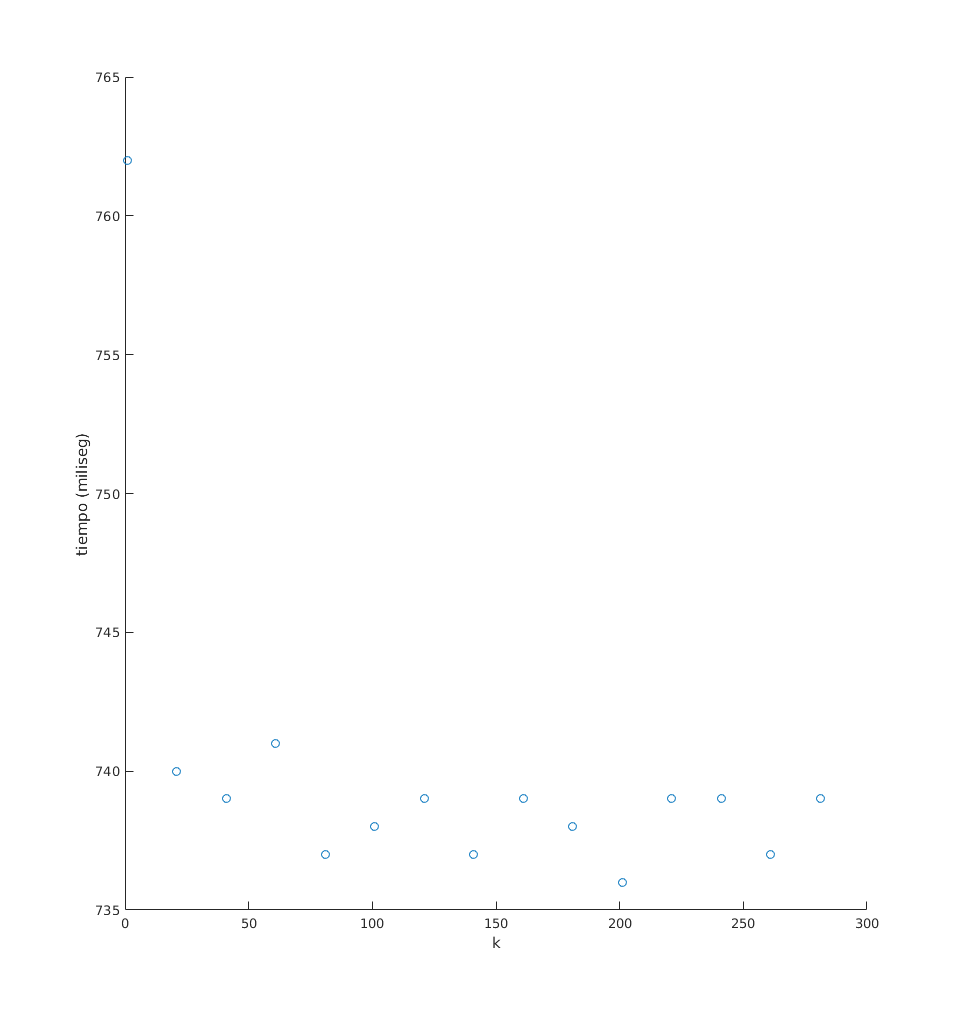
\includegraphics[width=\linewidth]{img/k_knn_tiempo.png}
\caption{Utilizando imágenes reducidas}
\end{subfigure}
\hfill
\begin{subfigure}[h]{0.62\linewidth}
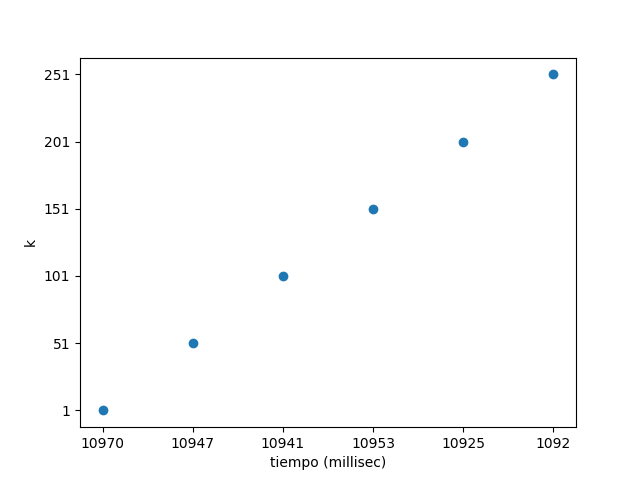
\includegraphics[width=\linewidth]{img/big_k_knn_tiempo.png}
\caption{Utilizando imágenes grandes}
\end{subfigure}%
\caption{Tiempo vs K con KNN sin PCA}
\end{figure}


En este caso no logramos identificar ningún patrón evidente. Si bien en el segundo gráfico se observan algúnas diferencias, en realidad representan pequeñas variaciones en el tiempo de ejecución que no consideramos relevantes.
Esto nos parece razonable, dado que por la forma de nuestra implementación calculamos la distancia con cada una de las imágenes y elegir un K mayor implica muy pocos cálculos adicionales.
%%%%%%%%%%%%%%%%%%%%%%%%%%%%%%%%%%%%%%%%%%%%%%%%%%%%%%%%%%%%%%%%%%%%%


\subsubsection*{Conclusiones del test}
Dados los resultados resulta evidente que cuánto más chico el K mejor se comportan nuestras métricas, luego concluímos que K = 1 es el valor óptimo.
Esto tiene sentido, sin embargo en caso de tener que implementar este problema en la vida real creemos que nos encontraríamos con outliers que pueden afectar el resultado, ya que con un solo vecino cercano tenemos un sistema poco robusto, por lo que elegiríamos un K un poco más grande pero cercano a 1.

%%%%%%%%%%%%%%%%%%%%%%%%%%%%%%%%%%%%%%%%%%%%%%%%%%%%%%%%%%%%%%%%%%%%%
\subsubsection*{Test con KNN + PCA}
Aquí evaluamos cómo se comporta nuestra implementación con PCA, para eso vamos a repetir los tests anteriores pero esta vez utilizando KNN+PCA.
De acuerdo a lo concluído de los tests anteriores inferimos que utilizar K = 1 o algún valor cercano sería lo mejor. 



%%%%%%%%%%%%%%%%%%%%%%%%%%%%%%%%%%%%%%%%%%%%%%%%%%%%%%%%%%%%%%%%%%%%%
\begin{figure}[H]
	\centering
	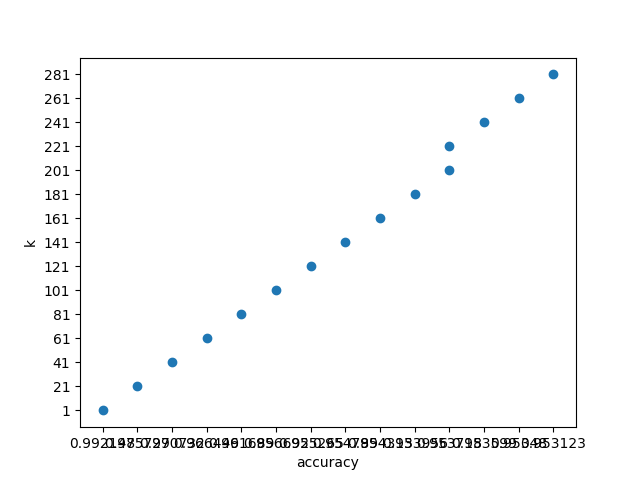
\includegraphics[width=0.8\textwidth]{img/k_pca_accu.png}
	\caption{Accuracy vs K con KNN + PCA}
	\label{fig:K vs Accuracy con KNN + PCA}
\end{figure}

En este caso observamos una estrecha relación entre cuántos vecinos cercanos tomamos y el Accuracy.
Nuevamente K = 1 parece ser el valor óptimo.

%%%%%%%%%%%%%%%%%%%%%%%%%%%%%%%%%%%%%%%%%%%%%%%%%%%%%%%%%%%%%%%%%%%%%

\begin{figure}[H]
\begin{subfigure}[h]{0.62\linewidth}
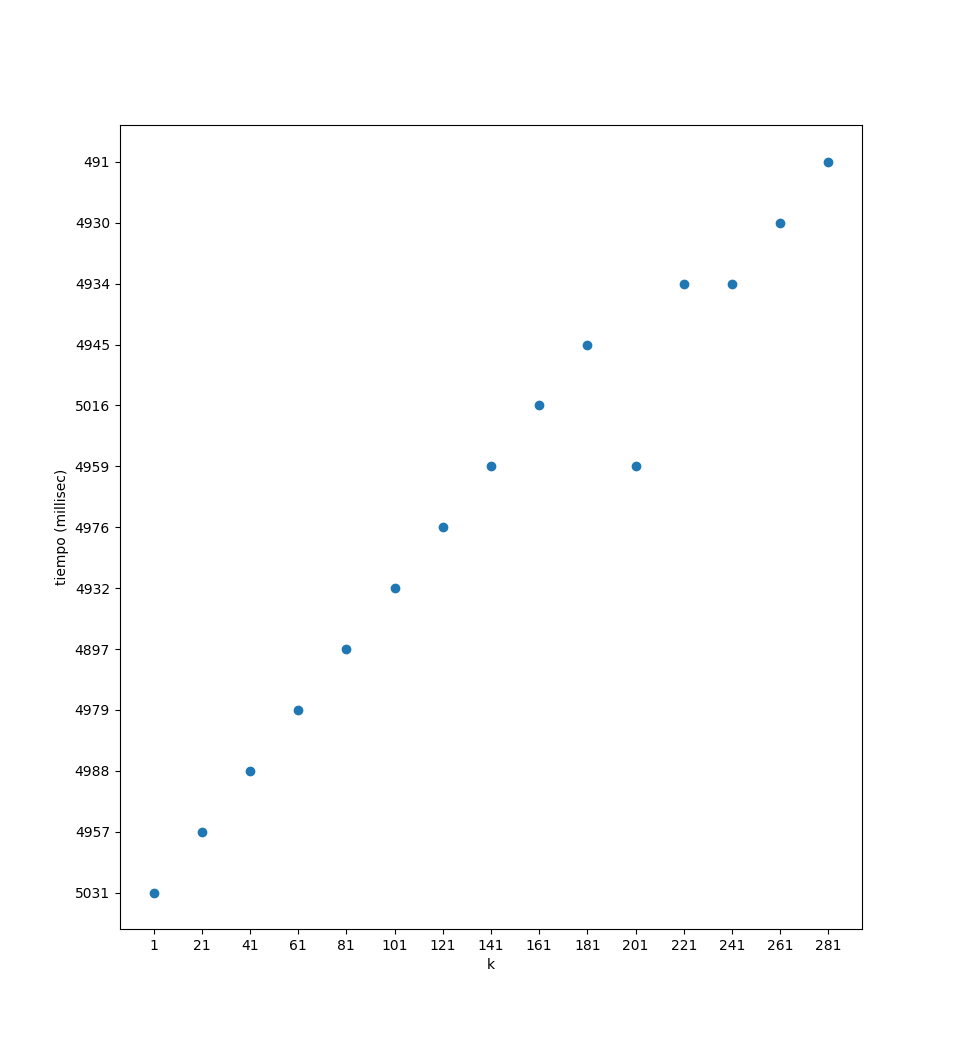
\includegraphics[width=\linewidth]{img/k_pca_tiempo.png}
\caption{Utilizando imágenes reducidas}
\end{subfigure}
\hfill
\begin{subfigure}[h]{0.62\linewidth}
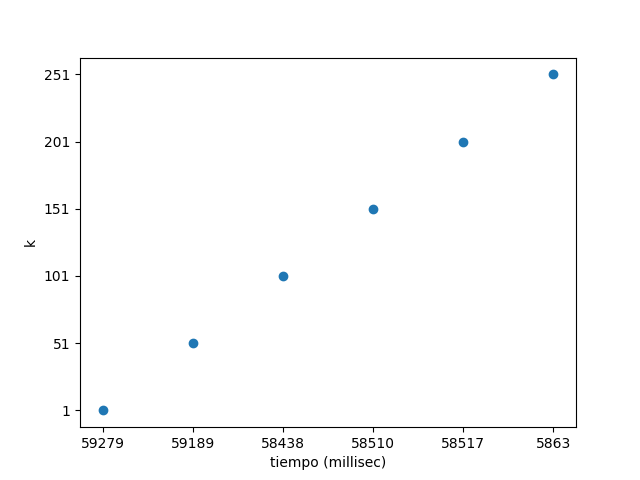
\includegraphics[width=\linewidth]{img/big_k_pca_tiempo.png}
\caption{Utilizando imágenes grandes}
\end{subfigure}%
\caption{Tiempo vs. K con KNN+PCA}
\end{figure}
Este caso es muy similar al visto sin PCA (Figura 3), no notamos diferencias relevantes.

Nótese que al calcular el tiempo incluimos desde el principio hasta el final del algoritmo. Para apreciar mejor la función de PCA tendríamos que haber calculado el tiempo del reconocimiento sin contar el cálculo de PCA. Este fue un hecho que notamos una vez terminada la experimentación pero sería un experimento interesante, que dejaremos para un futuro.\newline
Sin embargo vimos que PCA funciona correctamente en cuanto a nuestras métricas y por nuestra implementación, al trabajar con una matriz más chica obtendríamos una reducción en el tiempo de ejecución (tal como observamos al probar KNN sin PCA con el set de imágenes chico y el gránde), con esto podemos deducir que el reconocimiento una vez aplicado PCA tarda menos y a la vez sigue siendo efectivo.

%%%%%%%%%%%%%%%%%%%%%%%%%%%%%%%%%%%%%%%%%%%%%%%%%%%%%%%%%%%%%%%%%%%%%

\begin{figure}[H]
\begin{subfigure}[h]{0.62\linewidth}
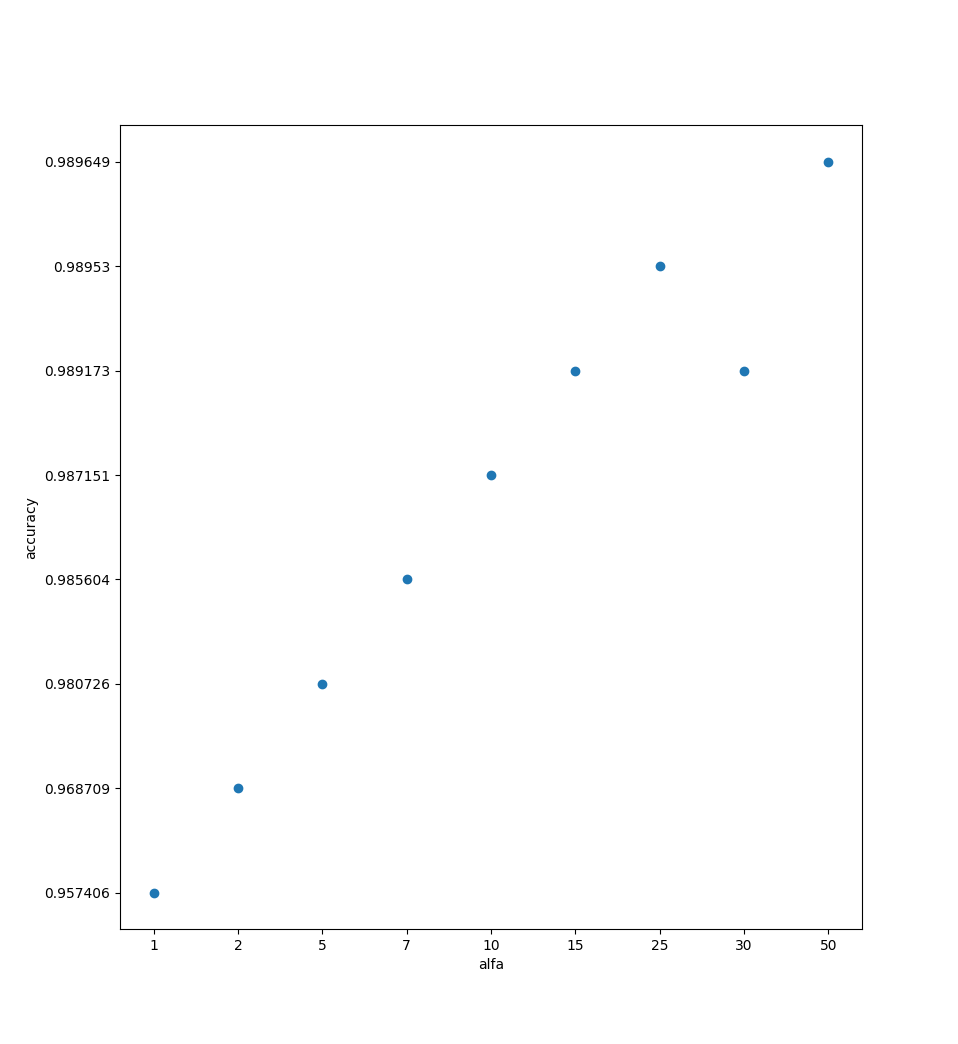
\includegraphics[width=\linewidth]{img/alfa_pca_accu.png}
\caption{Utilizando imágenes reducidas}
\end{subfigure}
\hfill
\begin{subfigure}[h]{0.62\linewidth}
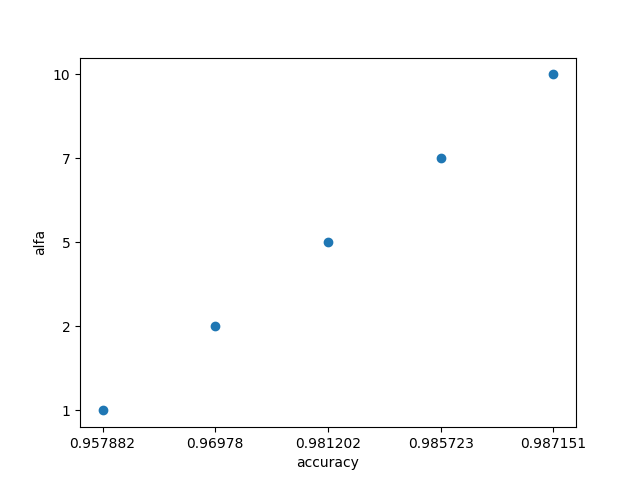
\includegraphics[width=\linewidth]{img/big_alfa_pca_accu.png}
\caption{Utilizando imágenes grandes}
\end{subfigure}%
\caption{Accuracy vs $\alpha$ con KNN+PCA}
\end{figure}

En este caso podemos observar una relación entre las dos variables, a medida que el $\alpha$ aumenta vemos como también lo hace nuestro accuracy.
Como expresamos anteriormente, debido al funcionamiento de PCA esperábamos que a mayor $\alpha$, obtendríamos una mejor reconstrucción y por lo tanto mejores resultados (en todas nuestras métricas en general).

Pero a su vez vimos que un $\alpha$ muy elevado resultaría en un aumento del tiempo de ejecución, no obstante en este gráfico vemos como las diferencias entre accuracy son cada vez menores, es decir como disminuye la pendiente (por ejemplo entre $\alpha$ = 10 y $\alpha$ = 50).

En base a los resultados obtenidos concluimos que un valor de $\alpha$ cercano a 10 nos daría un buen balance entre la cantidad de componentes principales y la efectividad (la cuál disminuye un poco, pero a cambio trabajamos con imágenes mucho más chicas).

Se puede ver en el gráfico a) que el valor máximo probado es $\alpha$ = 50 mientras que en el gráfico b) es $\alpha$ = 10. Esto se debe a que al trabajar en b) con imágenes más grandes requería mucho tiempo de ejecución ya que en los tests se realiza el preprocesamiento de las imágenes en cada corrida, por esto es que probamos solo hasta ese valor, donde igualmente podemos notar la forma del gráfico.

%%%%%%%%%%%%%%%%%%%%%%%%%%%%%%%%%%%%%%%%%%%%%%%%%%%%%%%%%%%%%%%%%%%%%
\begin{figure}[H]
\begin{subfigure}[h]{0.62\linewidth}
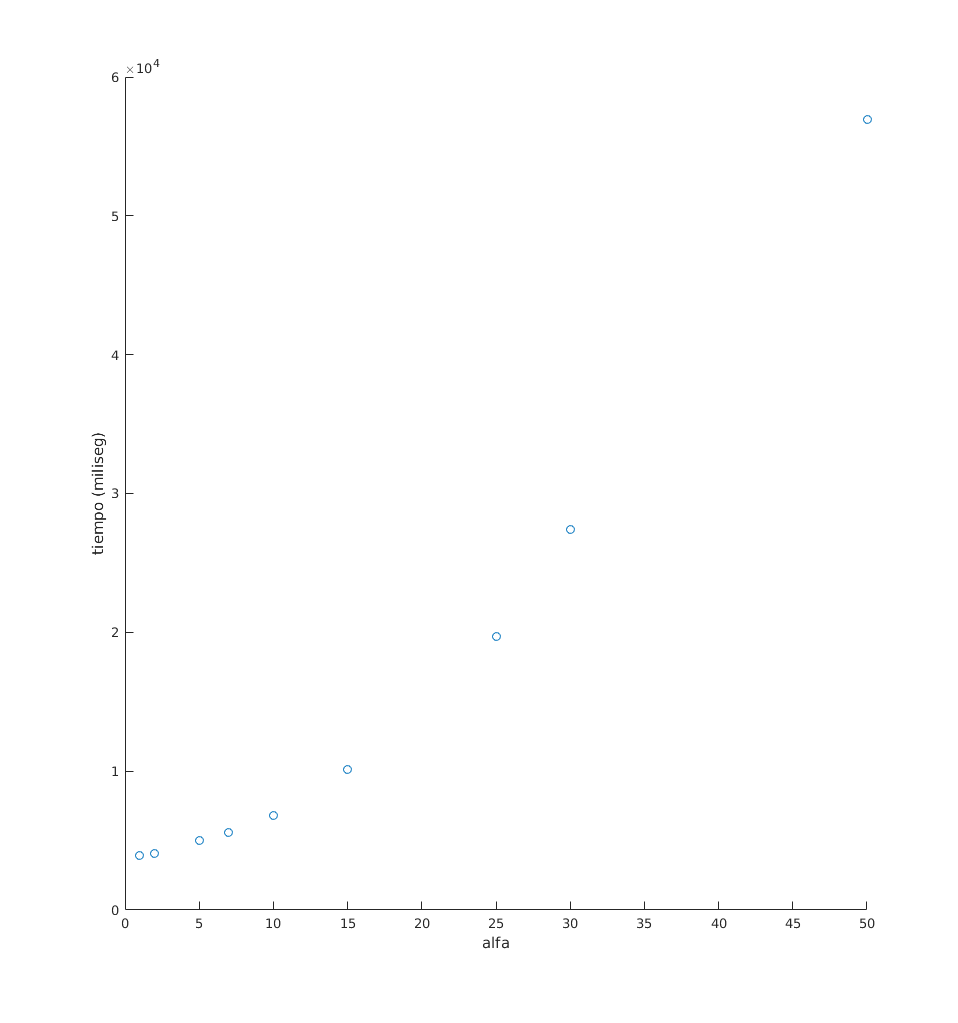
\includegraphics[width=\linewidth]{img/alfa_pca_tiempo.png}
\caption{Utilizando imágenes reducidas}
\end{subfigure}
\hfill
\begin{subfigure}[h]{0.62\linewidth}
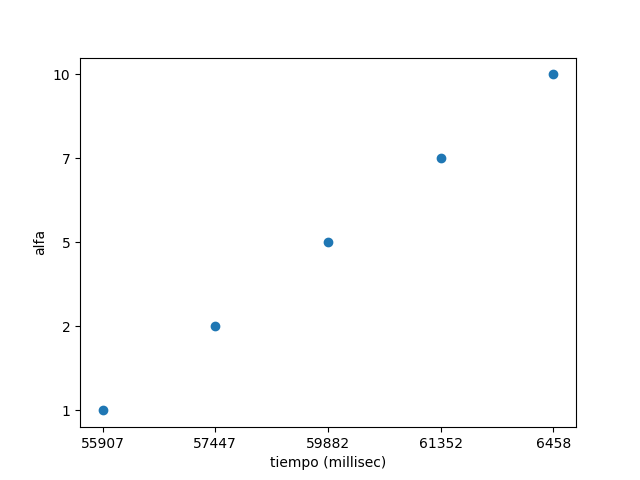
\includegraphics[width=\linewidth]{img/big_alfa_pca_tiempo.png}
\caption{Utilizando imágenes grandes}
\end{subfigure}%
\caption{Tiempo vs $\alpha$ con KNN+PCA}
\end{figure}

Tal como esperábamos vemos que a medida que el $\alpha$ aumenta (es decir, cuantas más componentes principales tengamos), el tiempo de ejecución también lo hace.

Luego, en línea con los resultados de los gráficos anteriores (Accuracy vs $\alpha$) podemos volver a afirmar que un $\alpha$ cercano a 10 sería un buen balance. En a) notamos que si tomáramos $\alpha$ = 30, tardaría aproximadamente el triple y no obtendríamos una mejora en el accuracy que valga la pena.
%%%%%%%%%%%%%%%%%%%%%%%%%%%%%%%%%%%%%%%%%%%%%%%%%%%%%%%%%%%%%%%%%%%%%
\begin{figure}[H]
	\centering
	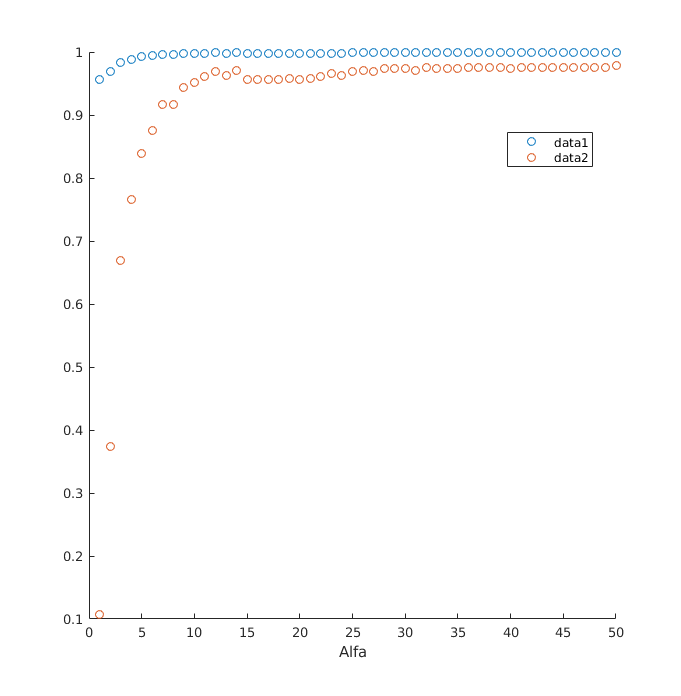
\includegraphics[width=0.8\textwidth]{img/Acc_recall_alfa_pca.png}
	\caption{Accuracy y Recall vs Alfa (con PCA)}
	\label{fig: Accuracy y Recall vs Alfa (con PCA)}
\end{figure}

En este caso al evaluar también recall observamos algo similar, a partir de 10 obtenemos un valor aceptable de esta métrica.
%%%%%%%%%%%%%%%%%%%%%%%%%%%%%%%%%%%%%%%%%%%%%%%%%%%%%%%%%%%%%%%%%%%%%

\begin{figure}[H]
	\centering
	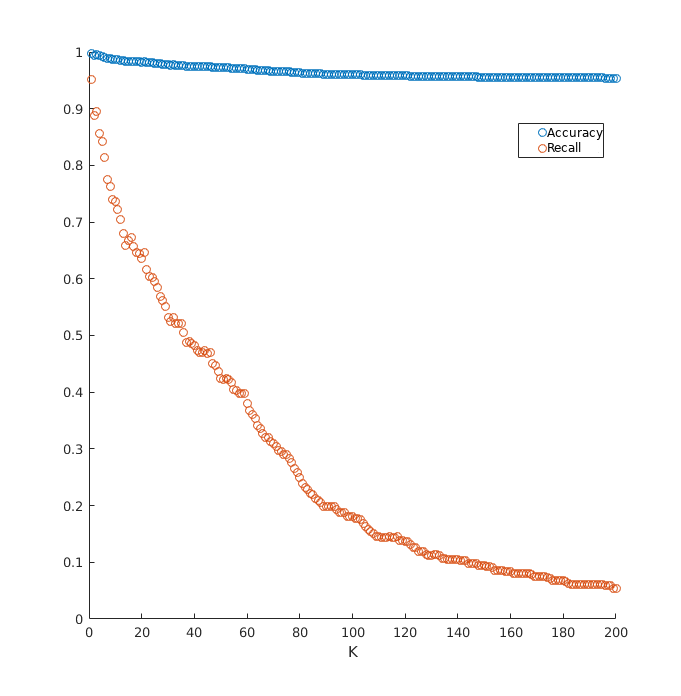
\includegraphics[width=0.8\textwidth]{img/Acc_recall_k_pca.png}
	\caption{Accuracy y Recall vs K (con PCA)}
	\label{fig: Accuracy y Recall vs K (con PCA)}
\end{figure}
Observamos que el resultado es realmente similar al del mismo test llevado a cabo sin PCA, luego por los mismos argumentos utilizados en el caso mencionado decimos que K = 1 es el mejor valor.
También podríamos agregar que el hecho de obtener resultados muy similares al test sin PCA habla bien del funcionamiento de PCA (con $\alpha$ = 10) que obtiene una buena tasa de reconocimiento con muy pocas componentes (lo que equivale a un gran ahorro de espacio).
%%%%%%%%%%%%%%%%%%%%%%%%%%%%%%%%%%%%%%%%%%%%%%%%%%%%%%%%%%%%%%%%%%%%%

Llegamos a la conclusión de que utilizando un valor de K cercano a 10 obtenemos la mejor relación (dentro de nuestro set de tests).
Por un lado evitamos el problema que ocurre cuando K es demasiado grande y por otro, tomamos una cantidad de imágenes cercanas suficiente como para minimizar el impacto de algún outsider.



\newpage


\section{Discusión}
Las expectativas que teníamos respecto de las pruebas usando solo KNN en comparación a KNN + PCA era que la segunda iba a dar mejores resultados en cuanto a las métricas de reconocimiento, sin embargo esto no fue así, lo que sí se logra usando PCA es trabajar con matrices más chicas, lo cual es útil si se trabaja con una base de datos con imágenes grandes o con muchas imágenes.
Con respecto a los tiempos tal como esperábamos PCA resulta lento en el procesamiento de la base de datos de entrenamiento sobre todo cuando se agregan muchas componentes principales. También suponíamos que las primeras componentes principales iban a influir más en tener buenos resultados de reconocimiento. Esto efectivamente fue así y lo usamos al diseñar los casos de test usando $\alpha$ más próximos en los valores pequeños y espaciándolos en valores más altos.
Una de las cosas que suponíamos es que usando un K más alto en KNN iba a funcionar mejor, pero esto no fue así, dando mejores métricas para K más chicos.
Los tiempos de ejecución fue una de las cuestiones que tuvimos en cuenta a a hora de diseñar los casos de pruebafundamentalmente en las corridas que usan PCA.
\newpage

\section{Conclusiones}
\subsubsection*{Conclusiones}

\newpage

\end{document}

